% questions.tex —— 2011 年·安徽卷·理科 · 题目内容片段（无答案）
% 由 tools/generate_projects.py 依来源总账自 2011/2011_数学真题_安徽理_试题.md 生成，勿手改（改源 MD 后重跑）


\gkpart{数学}

\begin{gktip}
\textbf{来源说明}：本题面依据固定源 PDF 两页 A3 题面逐栏转录（每页三栏），原卷印刷页码 643–644。固定源不附答案，原页各题与各节均未印分值，全部记「原页未标」，不补。答案与解析均由本库独立复算。

\textbf{源疑点}：第 6 题的三视图只见正视图与俯视图各标 $4$、俯视图左侧标 $1$、$2$、$1$，侧视图的梯形未标上底长度（解析按俯视图 $1+2+1$ 与侧视图拓扑补为 $2$，属由图上关系推得，非原页文字）。第 17 题的立体图中线段 $BF$ 在原页画作实线，本题各小问均未用到该线段，照录不改。第 21 题题面未排除 $B$ 与 $A$ 重合，此时 $P$ 与 $A$ 重合，仍在所求轨迹上，解析不另剔除（见解析正文）。第 20 题第（2）问的随机变量 $X$ 取「所需派出人员数目」，三人全部失败时亦记 $X=3$，原页未明示此约定，解析按此理解并注明。

\textbf{图形说明}：第 6、10、11、17、21 题的三视图、函数图象、程序框图、多面体、抛物线与向量条件均重绘为 TikZ 矢量图，依原页拓扑重绘，不按比例。
\end{gktip}

\gkpart{一、选择题}

\begin{question}
\gkti{1}设 $\mathrm i$ 是虚数单位，复数 $\dfrac{1+ai}{2-\mathrm i}$ 为纯虚数，则实数 $a$ 为\mbox{（　　）}

（A）$2$

（B）$-2$

（C）$-\frac12$

（D）$\frac12$

\end{question}
\begin{question}
\gkti{2}双曲线 $2x^2-y^2=8$ 的实轴长是\mbox{（　　）}

（A）$2$

（B）$2\sqrt2$

（C）$4$

（D）$4\sqrt2$

\end{question}
\begin{question}
\gkti{3}设 $f(x)$ 是定义在 $\mathbf R$ 上的奇函数，当 $x\leqslant 0$ 时，$f(x)=2x^2-x$，则 $f(1)=$\mbox{（　　）}

（A）$-3$

（B）$-1$

（C）$1$

（D）$3$

\end{question}
\begin{question}
\gkti{4}设变量 $x$，$y$ 满足 $|x|+|y|\leqslant 1$，则 $x+2y$ 的最大值和最小值分别为\mbox{（　　）}

（A）$1$，$-1$

（B）$2$，$-2$

（C）$1$，$-2$

（D）$2$，$-1$

\end{question}
\begin{question}
\gkti{5}在极坐标系中，点 $\left(2,\dfrac{\pi}{3}\right)$ 到圆 $\rho=2\cos\theta$ 的圆心的距离为\mbox{（　　）}

（A）$2$

（B）$\sqrt{4+\frac{\pi^2}{9}}$

（C）$\sqrt{1+\frac{\pi^2}{9}}$

（D）$\sqrt3$

\Needspace{0.4\textheight}
\end{question}
\begin{question}
\gkti{6}一个空间几何体的三视图如图所示，则该几何体的表面积为\mbox{（　　）}

（A）$48$

（B）$32+8\sqrt{17}$

（C）$48+8\sqrt{17}$

（D）$80$
\nopagebreak[4]
\begin{center}% 2011 年安徽卷理科第 6 题：几何体的三视图（正视图 4×4 正方形、侧视图梯形、俯视图 4×4 分 1–2–1）。
% 来源 PDF：普通高考/2011/2011安徽理.pdf，SHA-256 83dabf28711e3020c00f9fc73f3bf7be70f65fed94ab6ad5b6a39ac840820c0f。
% 原页：第 1 页（A3 三栏）第 1 栏中下部，书页码 643。
% 重绘依据：照原页布局——正（主）视图在左上，侧（左）视图在右上，俯视图在左下；
%   正视图为边长 4 的正方形，左侧与上方各标 4；侧视图为梯形，下底与原页同宽、上底约为其一半、高 4；
%   俯视图为 4×4 矩形，自上而下由两条横线分成 1、2、1 三段，左侧标 1、2、1。
%   原页未在侧视图上标上底长度，此处不补注数字；按原页拓扑与相对比例绘，不按原页绝对比例。
\begin{tikzpicture}[scale=0.95, >=stealth, semithick, font=\small]
  % 正视图（4×4）
  \draw (0,0) rectangle (4,4);
  % 侧视图（梯形：下底 4，上底 2，高 4）
  \draw (6,0) -- (10,0) -- (9,4) -- (7,4) -- cycle;
  % 俯视图（4×4，自上而下 1、2、1）
  \draw (0,-1.5) rectangle (4,-5.5);
  \draw (0,-2.5) -- (4,-2.5);
  \draw (0,-4.5) -- (4,-4.5);
  % 正视图尺寸标注
  \draw[<->] (0,4.42) -- (4,4.42) node[midway,above] {$4$};
  \draw[<->] (-0.52,0) -- (-0.52,4) node[midway,left] {$4$};
  % 俯视图尺寸标注
  \draw[<->] (-0.52,-1.5) -- (-0.52,-2.5) node[midway,left] {$1$};
  \draw[<->] (-0.52,-2.5) -- (-0.52,-4.5) node[midway,left] {$2$};
  \draw[<->] (-0.52,-4.5) -- (-0.52,-5.5) node[midway,left] {$1$};
  % 视图名称
  \node at (2,-0.65) {正（主）视图};
  \node at (8,-0.65) {侧（左）视图};
  \node at (2,-6.1) {俯视图};
\end{tikzpicture}
\end{center}
\nopagebreak[4]
\end{question}
\begin{question}
\gkti{7}命题“所有能被 $2$ 整除的整数都是偶数”的否定是\mbox{（　　）}

（A）所有不能被 $2$ 整除的整数都是偶数

（B）所有能被 $2$ 整除的整数都不是偶数

（C）存在一个不能被 $2$ 整除的整数是偶数

（D）存在一个能被 $2$ 整除的整数不是偶数

\end{question}
\begin{question}
\gkti{8}设集合 $A=\{1,2,3,4,5,6\}$，$B=\{4,5,6,7,8\}$，则满足 $S\subseteq A$ 且 $S\cap B\neq\varnothing$ 的集合 $S$ 的个数是\mbox{（　　）}

（A）$57$

（B）$56$

（C）$49$

（D）$8$

\end{question}
\begin{question}
\gkti{9}已知函数 $f(x)=\sin(2x+\varphi)$，其中 $\varphi$ 为实数，若 $f(x)\leqslant\left|f\left(\dfrac{\pi}{6}\right)\right|$ 对 $x\in\mathbf R$ 恒成立，且 $f\left(\dfrac{\pi}{2}\right)>f(\pi)$，则 $f(x)$ 的单调递增区间是\mbox{（　　）}

（A）$\left[k\pi-\frac{\pi}{3},k\pi+\frac{\pi}{6}\right]$（$k\in\mathbf Z$）

（B）$\left[k\pi,k\pi+\frac{\pi}{2}\right]$（$k\in\mathbf Z$）

（C）$\left[k\pi+\frac{\pi}{6},k\pi+\frac{2\pi}{3}\right]$（$k\in\mathbf Z$）

（D）$\left[k\pi-\frac{\pi}{2},k\pi\right]$（$k\in\mathbf Z$）

\Needspace{0.4\textheight}
\end{question}
\begin{question}
\gkti{10}函数 $f(x)=ax^m(1-x)^n$ 在区间 $[0,1]$ 上的图象如图所示，则 $m$，$n$ 的值可能是\mbox{（　　）}

（A）$m=1$，$n=1$

（B）$m=1$，$n=2$

（C）$m=2$，$n=1$

（D）$m=3$，$n=1$
\nopagebreak[4]
\begin{center}% 2011 年安徽卷理科第 10 题：函数 f(x)=a x^m (1-x)^n 在 [0,1] 上的图象。
% 来源 PDF：普通高考/2011/2011安徽理.pdf，SHA-256 83dabf28711e3020c00f9fc73f3bf7be70f65fed94ab6ad5b6a39ac840820c0f。
% 原页：第 1 页（A3 三栏）第 2 栏上部，书页码 643。
% 重绘依据：照原页——曲线自原点 O 陡升，在 x=0.5 略偏左处（约为 x=1/3）取最高点，最高点高度标为 0.5，
%   随后下降并在 x=1 处落回 x 轴；x 轴标 0.5 与 1，y 轴在 0.5 处有一短刻度并标 0.5。
%   取 a=27/8、m=1、n=2 作曲线（此时峰值 0.5 在 x=1/3 处取到），与原页示意一致；不按原页绝对比例。
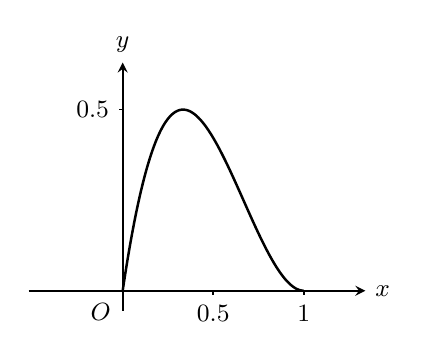
\begin{tikzpicture}[x=2.3cm, y=4.6cm, >=stealth, semithick, font=\small]
  % 坐标轴
  \draw[->] (-0.52,0) -- (1.34,0) node[right] {$x$};
  \draw[->] (0,-0.055) -- (0,0.63) node[above] {$y$};
  % 曲线 y=(27/8)x(1-x)^2
  \draw[line width=0.9pt] plot[domain=0:1, samples=140] (\x, {3.375*\x*(1-\x)*(1-\x)});
  % 刻度与标注
  \draw (-0.018,0.5) -- (0,0.5);
  \node[left] at (-0.02,0.5) {$0.5$};
  \draw (0.5,0) -- (0.5,-0.012);
  \node[below] at (0.5,-0.012) {$0.5$};
  \draw (1,0) -- (1,-0.012);
  \node[below] at (1,-0.012) {$1$};
  \node[below left] at (-0.01,-0.008) {$O$};
\end{tikzpicture}
\end{center}
\nopagebreak[4]
\end{question}
\gkpart{二、填空题}

\Needspace{0.4\textheight}
\begin{question}
\gkti{11}如图所示，程序框图（算法流程图）的输出结果是 $\underline{\qquad}$。
\nopagebreak[4]
\begin{center}% 2011 年安徽卷理科第 11 题：程序框图（算法流程图）。
% 来源 PDF：普通高考/2011/2011安徽理.pdf，SHA-256 83dabf28711e3020c00f9fc73f3bf7be70f65fed94ab6ad5b6a39ac840820c0f。
% 原页：第 1 页（A3 三栏）第 2 栏中部，书页码 643。
% 重绘依据：照原页——自上而下「开始」→ 矩形 T=0,k=0 → 矩形 T=T+k → 菱形 T>105?；
%   「是」向下经平行四边形「输出 k」到「结束」；「否」向右到矩形 k=k+1，
%   再上行折回、汇入 T=0,k=0 与 T=T+k 之间的竖直连线（原页箭头指入 T=T+k 上边）。
\begin{tikzpicture}[>=stealth, semithick, font=\small]
  \node[draw, rounded corners=0.12cm, minimum width=1.15cm, minimum height=0.50cm] (start) at (0,0) {开始};
  \node[draw, minimum width=2.05cm, minimum height=0.50cm] (init) at (0,-1.05) {$T=0,\ k=0$};
  \node[draw, minimum width=1.30cm, minimum height=0.50cm] (add) at (0,-2.00) {$T=T+k$};
  \node[draw, diamond, aspect=2.2, minimum width=2.10cm, minimum height=0.80cm] (test) at (0,-3.10) {$T>105$?};
  \node[draw, trapezium, trapezium left angle=70, trapezium right angle=110,
        minimum width=1.40cm, minimum height=0.55cm] (out) at (0,-4.30) {输出 $k$};
  \node[draw, rounded corners=0.12cm, minimum width=1.15cm, minimum height=0.50cm] (stop) at (0,-5.30) {结束};
  \node[draw, minimum width=1.20cm, minimum height=0.50cm] (inc) at (2.70,-3.10) {$k=k+1$};
  % 主干
  \draw[->] (start.south) -- (init.north);
  \draw[->] (init.south) -- (add.north);
  \draw[->] (add.south) -- (test.north);
  \draw[->] (test.south) -- (out.north) node[midway,right] {是};
  \draw[->] (out.south) -- (stop.north);
  % 「否」分支与回环
  \draw[->] (test.east) -- (inc.west) node[midway,above] {否};
  \draw (inc.north) -- (2.70,-1.55) -- (0,-1.55);
\end{tikzpicture}
\end{center}
\nopagebreak[4]
\end{question}
\begin{question}
\gkti{12}设 $(x-1)^{21}=a_0+a_1x+a_2x^2+\cdots+a_{21}x^{21}$，则 $a_{10}+a_{11}=$ $\underline{\qquad}$。

\end{question}
\begin{question}
\gkti{13}已知向量 $\boldsymbol a$，$\boldsymbol b$ 满足 $(\boldsymbol a+2\boldsymbol b)\cdot(\boldsymbol a-\boldsymbol b)=-6$，且 $|\boldsymbol a|=1$，$|\boldsymbol b|=2$，则 $\boldsymbol a$ 与 $\boldsymbol b$ 的夹角为 $\underline{\qquad}$。

\end{question}
\begin{question}
\gkti{14}已知 $\triangle ABC$ 的一个内角为 $120^\circ$，并且三边长构成公差为 $4$ 的等差数列，则 $\triangle ABC$ 的面积为 $\underline{\qquad}$。

\end{question}
\begin{question}
\gkti{15}在平面直角坐标系中，如果 $x$ 与 $y$ 都是整数，就称点 $(x,y)$ 为整点，下列命题中正确的是 $\underline{\qquad}$。（写出所有正确命题的编号）

① 存在这样的直线，既不与坐标轴平行又不经过任何整点；

② 如果 $k$ 与 $b$ 都是无理数，则直线 $y=kx+b$ 不经过任何整点；

③ 直线 $l$ 经过无穷多个整点，当且仅当 $l$ 经过两个不同的整点；

④ 直线 $y=kx+b$ 经过无穷多个整点的充分必要条件是：$k$ 与 $b$ 都是有理数；

⑤ 存在恰经过一个整点的直线。

\end{question}
\gkpart{三、解答题}

\begin{question}
\gkti{16}设 $f(x)=\dfrac{\mathrm e^x}{1+ax^2}$，其中 $a$ 为正实数。

（1） 当 $a=\dfrac43$ 时，求 $f(x)$ 的极值点；

（2） 若 $f(x)$ 为 $\mathbf R$ 上的单调函数，求 $a$ 的取值范围。

\Needspace{0.4\textheight}
\end{question}
\begin{question}
\gkti{17}如图，$ABEDFC$ 为多面体，平面 $ABED$ 与平面 $ACFD$ 垂直，点 $O$ 在线段 $AD$ 上，$OA=1$，$OD=2$，$\triangle OAB$，$\triangle OAC$，$\triangle ODE$，$\triangle ODF$ 都是正三角形。

（1） 证明直线 $BC\parallel EF$；

（2） 求棱锥 $F-OBED$ 的体积。
\nopagebreak[4]
\begin{center}% 2011 年安徽卷理科第 17 题：多面体 ABEDFC，平面 ABED ⊥ 平面 ACFD，O 在线段 AD 上，
%   OA=1，OD=2，△OAB、△OAC、△ODE、△ODF 均为正三角形。
% 来源 PDF：普通高考/2011/2011安徽理.pdf，SHA-256 83dabf28711e3020c00f9fc73f3bf7be70f65fed94ab6ad5b6a39ac840820c0f。
% 原页：第 1 页（A3 三栏）第 3 栏下部，书页码 643。
% 重绘依据：照原页——A 在左、D 在右，B 在 A 下方、E 在 D 下方，C 在 A 上方、F 在最上方偏左；
%   A、O、D 共线且在原页画作虚线；C、E、F 与 O 的连线（OC、OE、OF）在原页为虚线（被遮挡）；
%   AC、AB、BC、BE、BF、CF、EF、FD、ED 为实线，其中 BF 原页即画作实线，照录。
%   各点按原页投影位置取相对坐标，不按原页绝对比例。
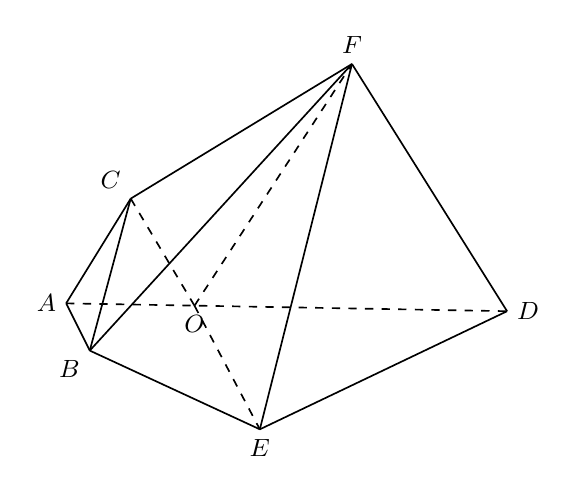
\begin{tikzpicture}[scale=1.0, >=stealth, semithick, font=\small]
  \coordinate (A) at (0,0);
  \coordinate (B) at (0.30,-0.60);
  \coordinate (C) at (0.82,1.33);
  \coordinate (O) at (1.63,-0.03);
  \coordinate (D) at (5.60,-0.10);
  \coordinate (E) at (2.46,-1.60);
  \coordinate (F) at (3.63,3.04);
  % 被遮挡的线
  \draw[dashed] (A) -- (D);
  \draw[dashed] (O) -- (C);
  \draw[dashed] (O) -- (E);
  \draw[dashed] (O) -- (F);
  % 可见的棱
  \draw (A) -- (C);
  \draw (A) -- (B);
  \draw (C) -- (B);
  \draw (B) -- (F);
  \draw (B) -- (E);
  \draw (C) -- (F);
  \draw (E) -- (F);
  \draw (F) -- (D);
  \draw (E) -- (D);
  % 顶点标注
  \node[left] at (A) {$A$};
  \node[below left] at (B) {$B$};
  \node[above left] at (C) {$C$};
  \node[below] at (O) {$O$};
  \node[right] at (D) {$D$};
  \node[below] at (E) {$E$};
  \node[above] at (F) {$F$};
\end{tikzpicture}
\end{center}
\nopagebreak[4]
\end{question}
\begin{question}
\gkti{18}在数 $1$ 和 $100$ 之间插入 $n$ 个实数，使得这 $n+2$ 个数构成递增的等比数列，将这 $n+2$ 个数的乘积记作 $T_n$，再令 $a_n=\lg T_n$，$n\geqslant 1$。

（1） 求数列 $\{a_n\}$ 的通项公式；

（2） 设 $b_n=\tan a_n\cdot\tan a_{n+1}$，求数列 $\{b_n\}$ 的前 $n$ 项和 $S_n$。

\end{question}
\begin{question}
\gkti{19}

（1） 设 $x\geqslant 1$，$y\geqslant 1$，证明 $x+y+\dfrac{1}{xy}\leqslant\dfrac1x+\dfrac1y+xy$；

（2） $1<a\leqslant b\leqslant c$，证明 $\log_a b+\log_b c+\log_c a\leqslant\log_b a+\log_c b+\log_a c$。

\end{question}
\begin{question}
\gkti{20}工作人员需进入核电站完成某项具有高辐射危险的任务，每次只派一个人进去，且每个人只派一次，工作时间不超过 $10$ 分钟，如果前一个人 $10$ 分钟内不能完成任务则撤出，再派下一个人。现在一共只有甲、乙、丙三个人可派，他们各自能完成任务的概率分别 $p_1$，$p_2$，$p_3$，假设 $p_1$，$p_2$，$p_3$ 互不相等，且假定各人能否完成任务的事件相互独立。

（1） 如果按甲最先，乙次之，丙最后的顺序派人，求任务能被完成的概率。若改变三个人被派出的先后顺序，任务能被完成的概率是否发生变化？

（2） 若按某指定顺序派人，这三个人各自能完成任务的概率依次为 $q_1$，$q_2$，$q_3$，其中 $q_1$，$q_2$，$q_3$ 是 $p_1$，$p_2$，$p_3$ 的一个排列，求所需派出人员数目 $X$ 的分布列和均值（数学期望）$EX$；

（3） 假定 $1>p_1>p_2>p_3$，试分析以怎样的先后顺序派出人员，可使所需派出的人员数目的均值（数学期望）达到最小。

\Needspace{0.4\textheight}
\end{question}
\begin{question}
\gkti{21}设 $\lambda>0$，点 $A$ 的坐标为 $(1,1)$，点 $B$ 在抛物线 $y=x^2$ 上运动，点 $Q$ 满足 $\overrightarrow{BQ}=\lambda\overrightarrow{QA}$，经过点 $Q$ 与 $x$ 轴垂直的直线交抛物线于点 $M$，点 $P$ 满足 $\overrightarrow{QM}=\lambda\overrightarrow{MP}$，求点 $P$ 的轨迹方程。
\nopagebreak[4]
\begin{center}% 2011 年安徽卷理科第 21 题：抛物线 y=x^2，A(1,1)，B 在抛物线上，BQ=λQA，
%   过 Q 作 x 轴垂线交抛物线于 M，QM=λMP。
% 来源 PDF：普通高考/2011/2011安徽理.pdf，SHA-256 83dabf28711e3020c00f9fc73f3bf7be70f65fed94ab6ad5b6a39ac840820c0f。
% 原页：第 2 页（A3 三栏）第 3 栏上部，书页码 644。
% 重绘依据：照原页——抛物线 y=x^2，A(1,1) 在右支上，B 在左支上（高于 A），
%   直线 BA 与 y 轴相交后向右下延伸过 A；Q 在 BA 上、位于 y 轴右侧，M 为过 Q 的竖直线与抛物线的交点，
%   P 在该竖直线上、位于 M 下方并以实心点标出；竖直线上端越过 Q 继续向上、下端伸到 x 轴下方。
%   x 轴上标 -1 与 1，y 轴在 y=1 处有刻度并标 1。取 B=(-1.15,1.3225)，Q、M、P 按解析式算得，
%   P 落在 y=2x-1 上；不按原页绝对比例。
\begin{tikzpicture}[x=2.1cm, y=2.1cm, >=stealth, semithick, font=\small]
  % 坐标轴
  \draw[->] (-1.70,0) -- (1.70,0) node[right] {$x$};
  \draw[->] (0,-1.05) -- (0,2.45) node[above] {$y$};
  % 抛物线
  \draw[line width=0.9pt] plot[domain=-1.549:1.549, samples=160] (\x, {\x*\x});
  % 竖直虚线所在直线（过 Q 的竖直线，原页为实线）
  \draw (0.45,-0.95) -- (0.45,2.30);
  % 直线 BA
  \draw (-1.15,1.3225) -- (1.16,0.9760);
  % 点
  \coordinate (A) at (1,1);
  \coordinate (B) at (-1.15,1.3225);
  \coordinate (Q) at (0.45,1.0825);
  \coordinate (M) at (0.45,0.2025);
  \coordinate (P) at (0.45,-0.10);
  \fill (P) circle (1.3pt);
  % 刻度
  \draw (-0.035,1) -- (0,1);
  \node[left] at (-0.05,1) {$1$};
  \draw (-1,0) -- (-1,-0.035);
  \node[below] at (-1,-0.045) {$-1$};
  \draw (1,0) -- (1,-0.035);
  \node[below] at (1,-0.045) {$1$};
  % 标注
  \node[below left] at (-0.04,-0.02) {$O$};
  \node[right] at (A) {$A$};
  \node[left] at (B) {$B$};
  \node[right] at (Q) {$Q$};
  \node[left] at (M) {$M$};
  \node[left] at (P) {$P$};
\end{tikzpicture}
\end{center}
\nopagebreak[4]

\end{question}